\chapter{Methodology}

%Algorithm training process:
%\begin{enumerate}
%\item Plants in the imagery will be localized with Faster R-CNN \cite{r-cnn} and cropped
%\item Localized plants will be associated with plant ID
%\item Cropped images will be used as training data, where targets are the plant health indicators
%\end{enumerate}

\section{Dataset Creation}
In this section, we go over the instruments and the process that we used to create the dataset.

\subsection{Instruments}
For the UAV, we utilized two different systems: Aibotix's Aibot X6 and PrecisionHawk's Lancaster 5 as pictured in Figures \ref{aibotx6} and \ref{lancaster5}. The Aibot X6 is a multirotor UAV equipped with a Headwall Nano-Hyperspec sensor. The Lancaster 5 is a fixed-wing UAV equipped with both a multispectral sensor and an RGB sensor.


\begin{figure}
    \centering
    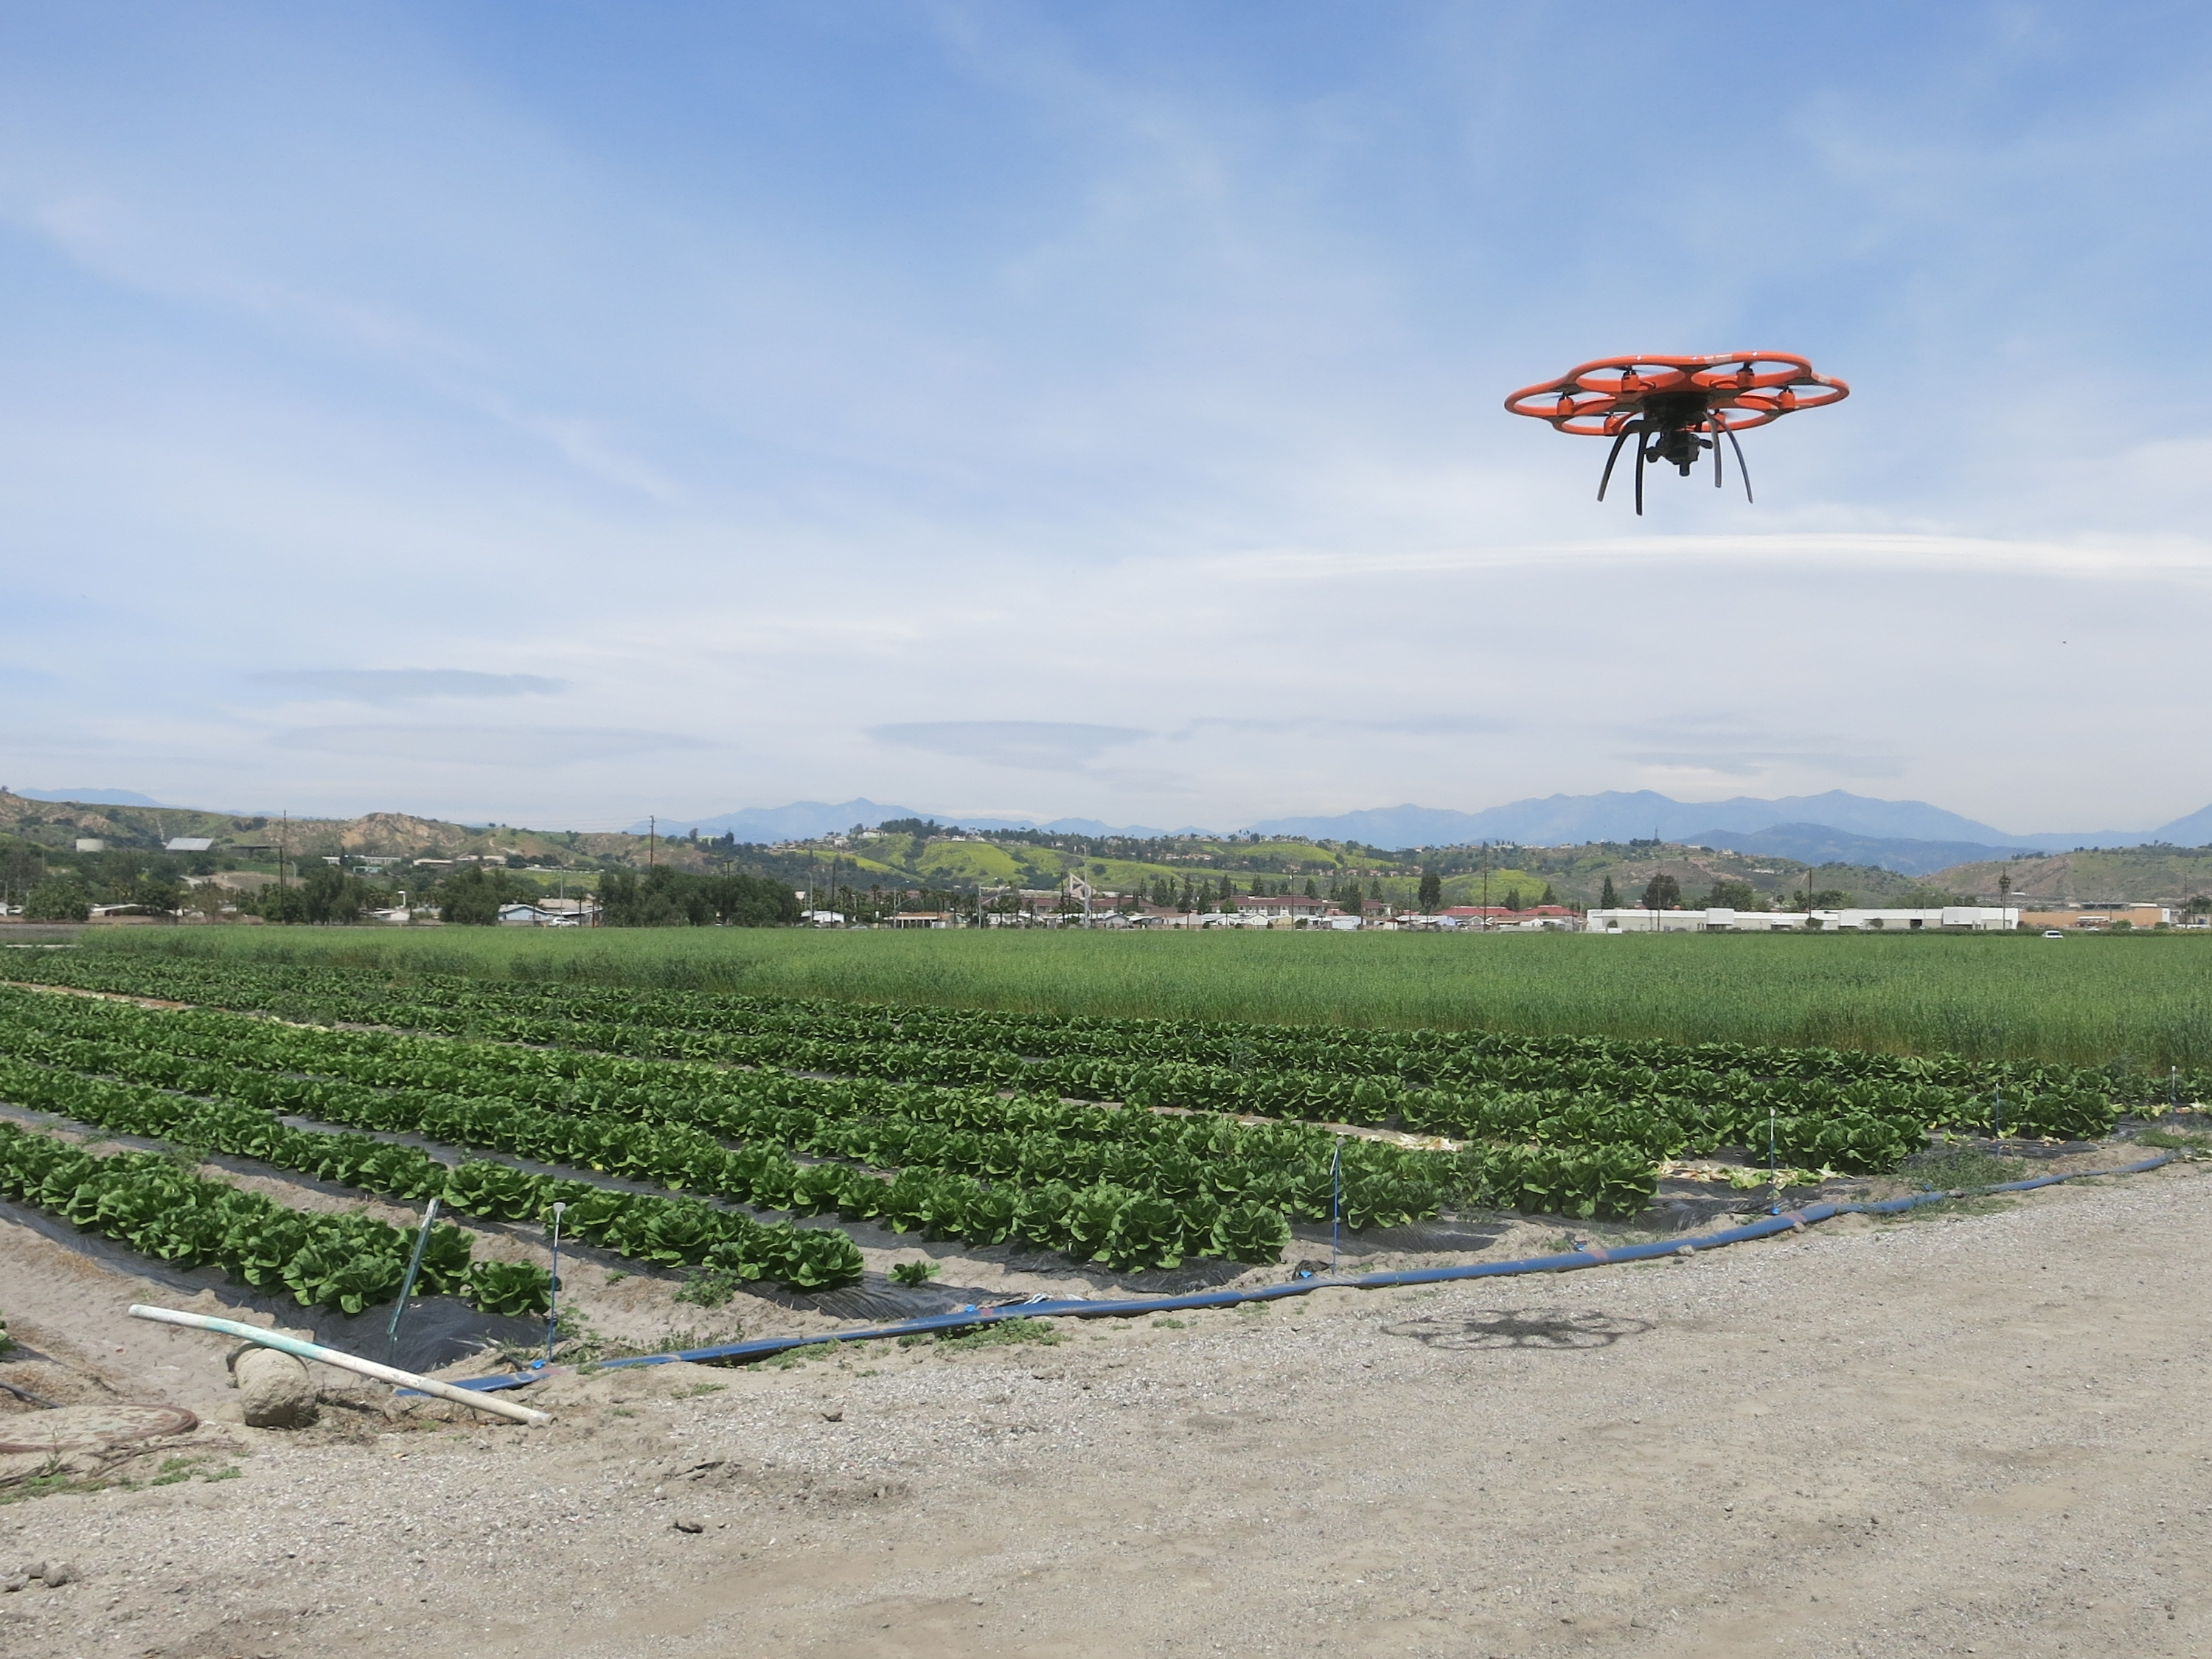
\includegraphics[width=0.8\textwidth]{images/aibotx6.JPG}
    \caption{Aibot X6 from Aibotix collecting data from our lettuce crops.}
    \label{aibotx6}
\end{figure}
\begin{figure}
    \centering
    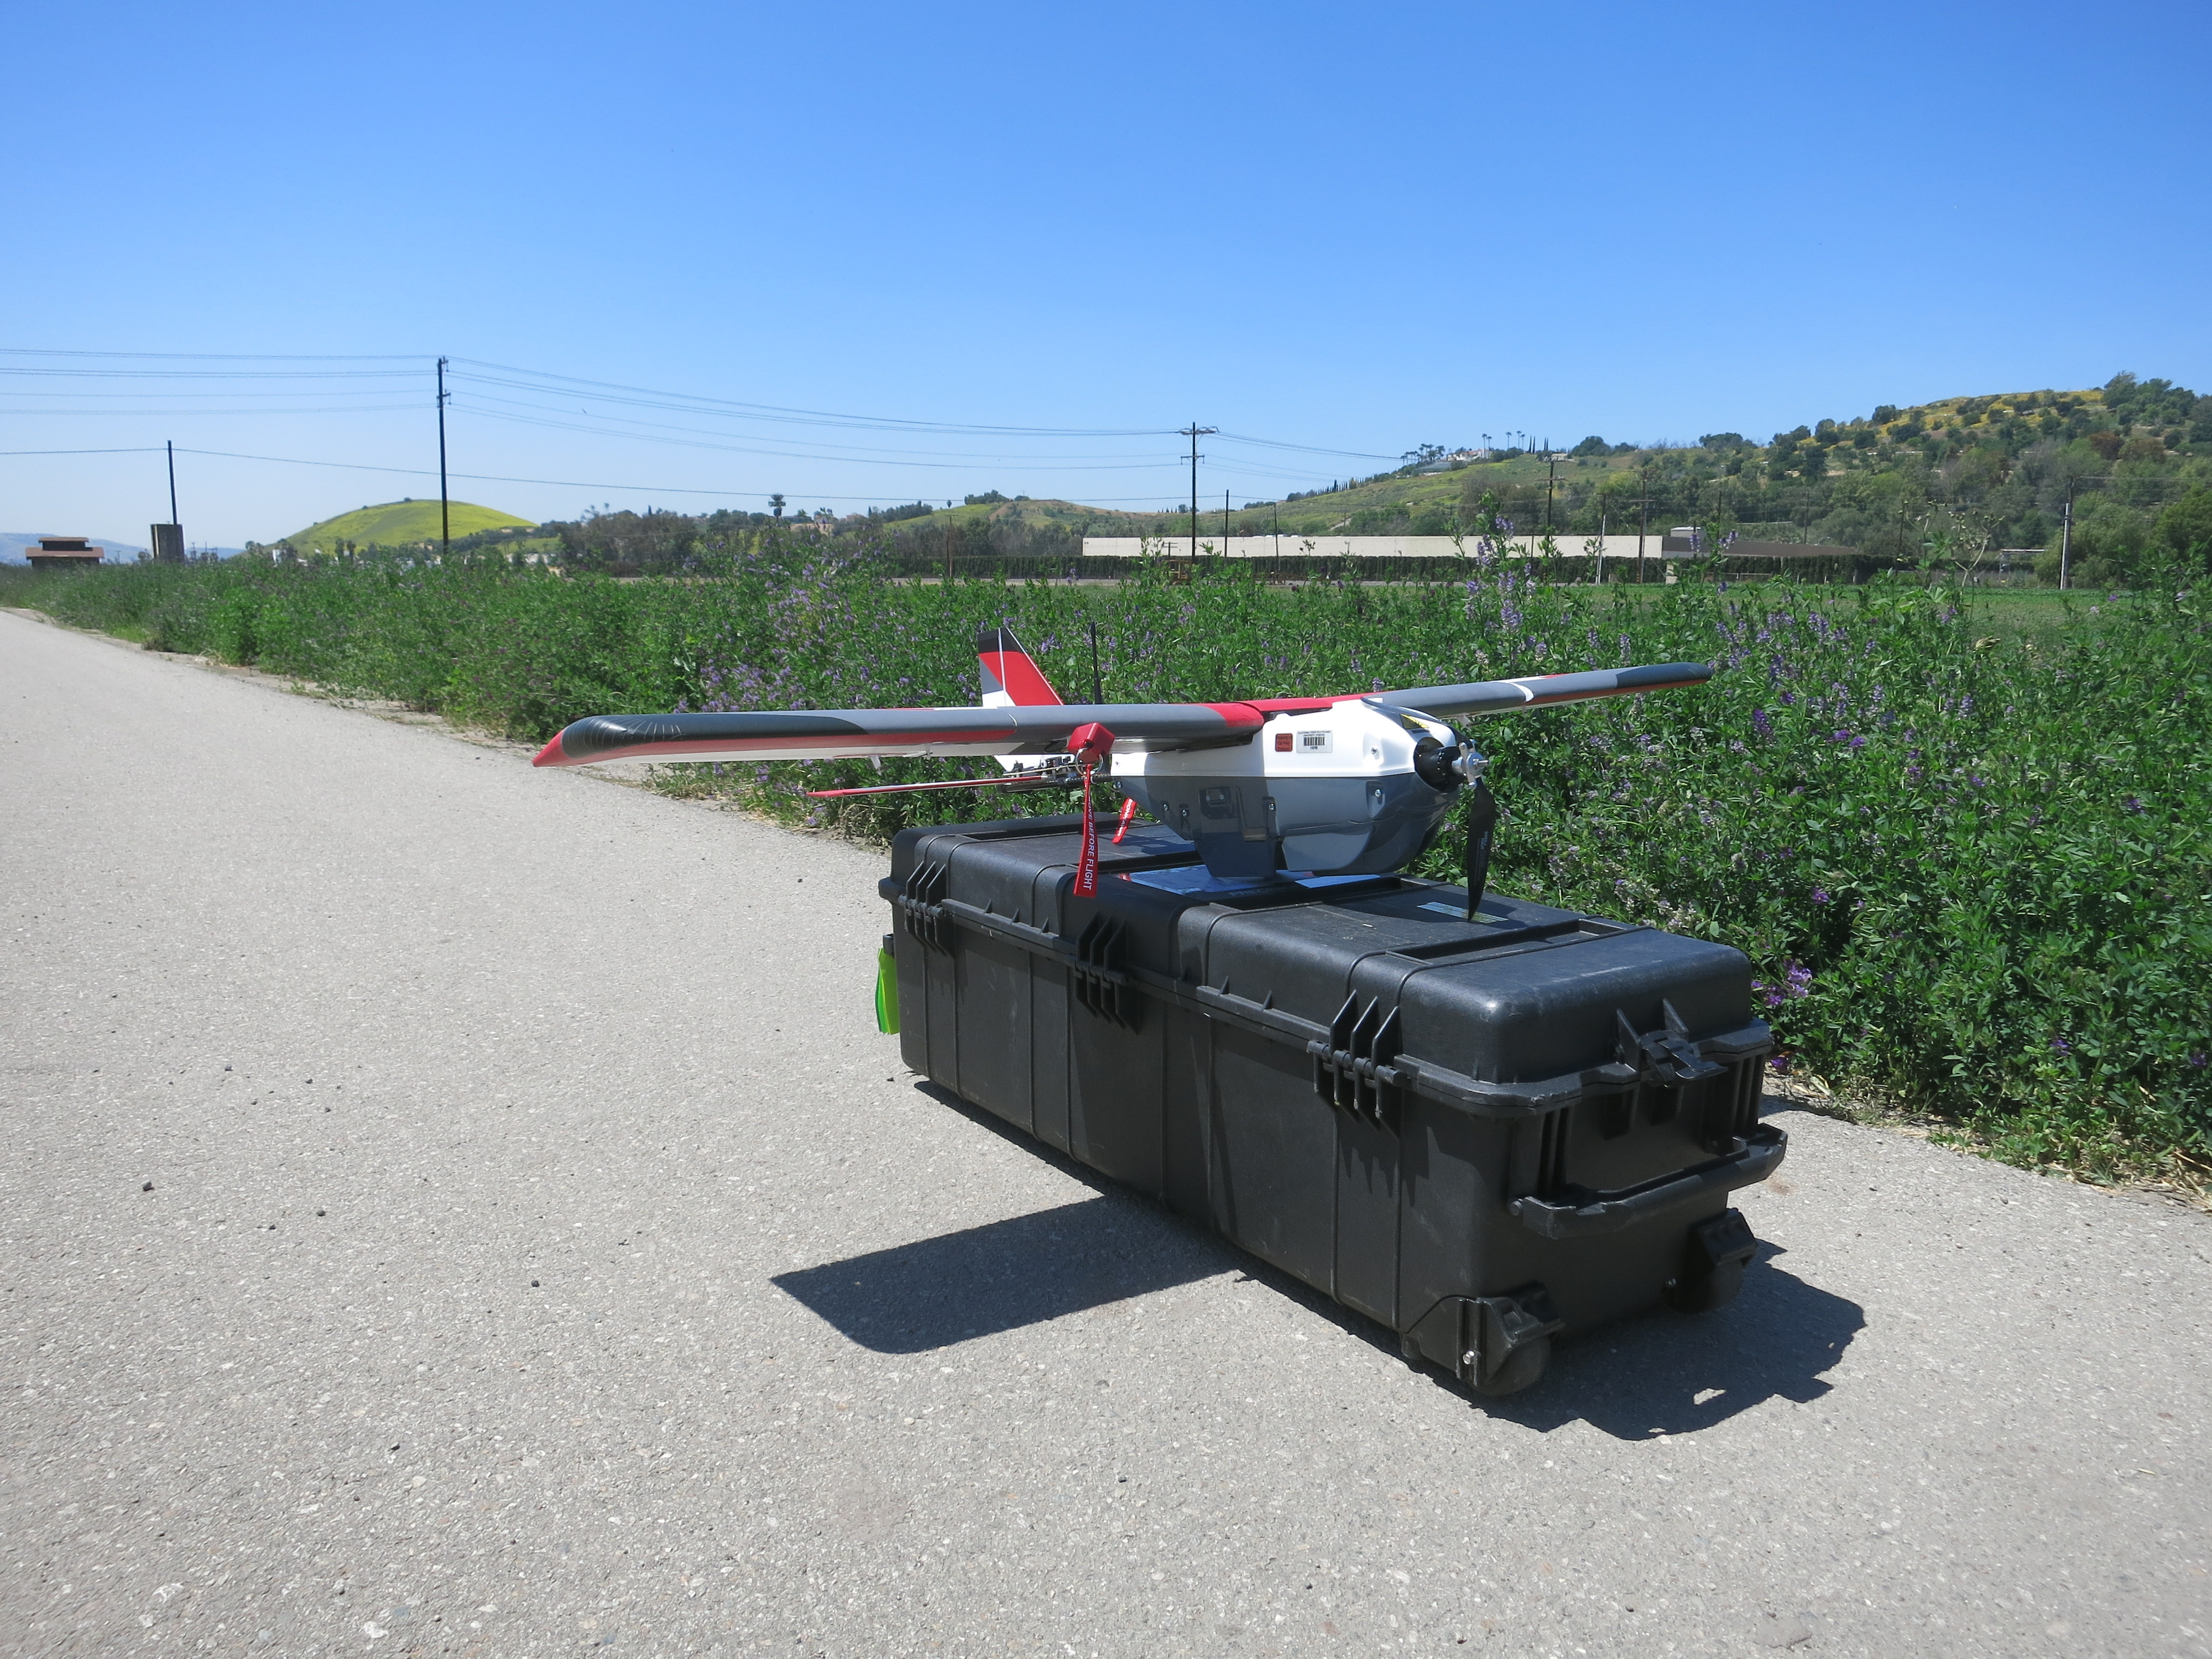
\includegraphics[width=0.8\textwidth]{images/lancaster5.JPG}
    \caption{Lancaster 5 from PrecisionHawk.}
    \label{lancaster5}
\end{figure}

To validate the multispectral data from the UAV, we used an ASD HandHeld 2 Spectroradiometer. We used the optional leaf clip attachment for more precise measurements.

To collect chlorophyll data, we used the Konica Minolta SPAD 502. It is a handheld device that measures the amount of chlorophyll in leaves, an indicator of how well fertilized a plant is.

The water potential data was determined using the Decagon WP4C. Leaf cutlets are inserted into the device where the readings are determined. The data is an indicator of how well the plant is being watered.



\subsection{Crop Treatment}
The lettuce plants were subjected to 16 different irrigation and nitrogen treatments. The irrigation levels were 0\%, 25\%, 50\% and 100\% of required water according to evapotranspiration. The nitrogen levels were 0\%, 25\%, 50\% and 100\% of required amount for optimal lettuce growth based on soil chemical analysis. This results in the 16 different treatments from the combinations of the 4 levels of irrigation and nitrogen. Each treatment had 3 replications giving us 48 experimental plots as seen in Figure \ref{lettuce_plot}.


\begin{figure}
    \centering
    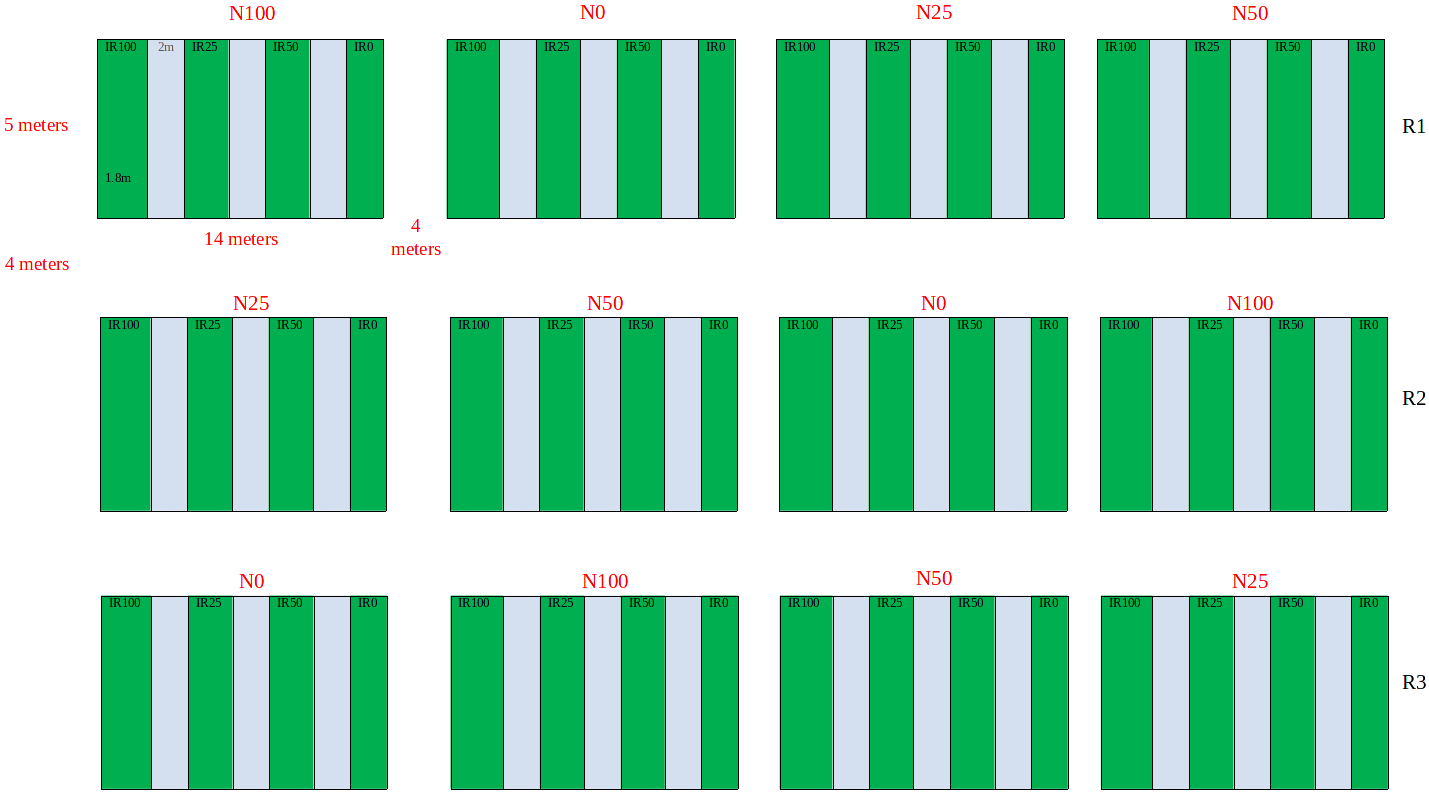
\includegraphics[width=1.0\textwidth]{images/plot.png}
    \caption{Experimental design of lettuce plot.}
    \label{lettuce_plot}
\end{figure}

\subsection{Data Collection Process}
Data was collected weekly at around noon as having direct sunlight is optimal for the remote sensing data. For the ground truthing data, we sampled 2 plants from each plot giving us data on 96 plants total.
With these 96 plants, we collect data from them using a handheld RGB camera, spectroradiometer, and chlorophyll meter. Since the water potential meter takes more time to process each sample than the other sensors, we were only able to get 1 sample per plot per week, resulting in 48 samples per week. % Plant height, soil moisture, mass

\subsection{UAV Image Processing}
As there are discrepancies in the UAV images due to inaccuracies in the GPS sensor and usage of multiple sensors, processing of the images is necessary. The first step of this process is to perform georeferencing in QGIS. This step will ensure that the coordinates embedded in the GeoTIFF images are properly aligned with the objects in the image. Using a manually generated shapefile, we crop the images so that they all display the same area. With these cropped images, we rotate them so that the rows of lettuce are horizontal. Finally, we resize the images to the dimensions of the smallest image.


\section{Models}

\subsection{Ground Truth Predictor}
With this model, we experiment with the various architectures listed previously: VGG, ResNet, DenseNet, and Inception. We utilize a pre-trained network and replace the final layers with our own.

\subsection{NDVI Predictor}
The goal of this model is to take as input an aerial RGB image and return an image of the same dimensions where each pixel value represents the level of NDVI. For this model, we modify FC-DenseNet so that it predicts a value from $[0, 256)$, which is a binned representation of the NDVI value.